\section{Advection - High Resolution}
\label{sec:module_advection}
% Define box and box title style
\tikzstyle{mybox} = [draw=black, fill=RUBgrau!20, very thick, rectangle, rounded corners, inner sep=10pt, inner ysep=20pt]
\tikzstyle{fancytitle} =[fill=RUBblau!100, text=white, rectangle, rounded corners,draw=black]

\begin{tikzpicture}
\node[mybox] (box)
{
  \begin{minipage}{1\textwidth}
  \begin{description}
  \item[Header file] AdvectionHR/AdvectionHR.h
  \item[What it does] Advects data in a Storage3D according to a given velocity field.
  \item[Requires] \nameref{sec:module_settings}, \nameref{sec:module_velocity}, \nameref{sec:module_boundaryconditions}
  \item[Input file] Advection.opi
  \item[Examples] /benchmarks/AdvectionHR, ...
  \end{description}
  \end{minipage}
};
\node[fancytitle, right=12pt] at (box.north west) {Module in brief...};
\end{tikzpicture}
\paragraph{Background and usage} Passive fields $q$ like temperature, concentrations and density are advected with velocity $v$ according to the advection equation
\begin{align}
\partial_t q + \nabla \cdot (qv) = 0.
\end{align}
Advection in each grid axis is handled individually as this allows for larger time steps due to the CFL-condition. Therefore we can simplify the problem to the one-dimensional case.
A Godunov-type scheme is utilized that considers the fluxes $f_{i+\frac{1}{2}}$ and $f_{i-\frac{1}{2}}$ over the border of a control volume
\begin{align}
q_i^{n+1} = q_i^n - \frac{dt}{dx}\left[f_{i+\frac{1}{2}}(t^n,q^n)-f_{i-\frac{1}{2}}(t^n,q^n)\right],
\end{align}
using the high resolution fluxes
\begin{align}
f_{i+\frac{1}{2}}(t,q) &= v^+(x_{i+\frac{1}{2}},t)\left[q_i+\phi\left(r_i\right)\left(q_{i+1}-q_i\right)\right]\\ \label{eq:advf}
                       &+ v^-(x_{i+\frac{1}{2}},t)\left[q_i+\phi\left(\frac{1}{r_{i+1}}\right)\left(q_{i}-q_{i+1}\right)\right],
\end{align}
with $v^+(x_{i+\frac{1}{2}},t) = \text{max}(\frac{v_{i+1}+v_i}{2},0)$ and $v^-(x_{i+\frac{1}{2}},t) = \text{min}(\frac{v_{i+1}+v_i}{2},0)$ and a flux limiter function $\phi$. that with a proper choice allows second order accuracy in smooth regions and counteracts oscillations near discontinuities as observed with second-order accurate methods such as Lax-Wendroff or Beam-Warming, see \citeopref{leveque.r.2002}. The quotient $r_i$ is determined by two consecutive slopes as
\begin{align}
r_i = \frac{q_i-q_{i-1}}{q_{i+1}-q_i}.
\end{align}
In order to avoid a division by zero when $q_{i+1} = q_i$ we replace the limited slopes in \ref{eq:advf} with
\begin{align}
\phi(r_i)(q_{i+1}-q_i) &= L(q_{i+1}-q_i,q_i-q_{i-1}),\\
\phi\left(\frac{1}{r_{i+1}}\right)\left(q_{i}-q_{i+1}\right) &= -L(q_{i+2}-q_{i+1},q_{i+1}-q_{i}),
\end{align}
as suggested in \citeopref{jameson.a.1995}. 
The limiters implemented in OpenPhase are\\
\\
\begin{tabular}{ll}
Minmod: & $L(a,b) := S(a,b)\text{min}\left(\left|a\right|,\left|b\right|\right)$, \\
Monotonized Central: & $L(a,b) := S(a,b)\text{min}\left(\frac{\left|a+b\right|}{2},2\left|a\right|,2\left|b\right|\right)$, \\
Superbee: & $L(a,b) := S(a,b)\text{max}\left(\text{min}\left(2\left|a\right|,\left|b\right|\right),\text{min}\left(\left|a\right|,2\left|b\right|\right)\right)$, \\
\end{tabular} 
\\
\\
with
\begin{align}
S(a,b) := \frac{\text{sgn}(a)+\text{sgn}(b)}{4}.
\end{align}
In the case of $L(a,b) = 0$ for all $a,b \in \mathbb{R}$ the scheme becomes a simple first-order upwind method.
Finally we have
\begin{align}
f_{i+\frac{1}{2}}(t,q) &= v^+(x_{i+\frac{1}{2}},t)\left[q_i+L(q_{i+1}-q_i,q_i-q_{i-1})\right]\\
                       &+ v^-(x_{i+\frac{1}{2}},t)\left[q_i-L(q_{i+2}-q_{i+1},q_{i+1}-q_{i})\right],\\
f_{i-\frac{1}{2}}(t,q) &= v^+(x_{i-\frac{1}{2}},t)\left[q_{i-1}+L(q_{i}-q_{i-1},q_{i-1}-q_{i-2})\right]\\
                       &+ v^-(x_{i-\frac{1}{2}},t)\left[q_{i-1}-L(q_{i+1}-q_{i},q_{i}-q_{i-1})\right].
\end{align}
For multi-dimensional system those one dimensional-advection methods are used subsequently in each direction. The Strang splitting technique, which alternates order of execution in each time step, is second order accurate in time \citeopref{leveque.r.2002}.
For $n \text{ mod } 2 = 0$ the schemes becomes
\begin{align}
q^{n+\frac{1}{3}} &= q^n - dt(v_1q^n)_x^h, \\
q^{n+\frac{2}{3}} &= q^{n+\frac{1}{3}} - dt(v_2q^{n+\frac{1}{3}})_y^h, \\
q^{n+1} &= q^{n+\frac{2}{3}} - dt(v_3q^{n+\frac{2}{3}})_z^h, \\
q^{n+1+\frac{1}{3}} &= q^{n+1} - dt(v_3q^{n+1})_z^h, \\
q^{n+1+\frac{2}{3}} &= q^{n+1+\frac{1}{3}} - dt(v_2q^{n+1+\frac{1}{3}})_y^h, \\
q^{n+2} &= q^{n+1+\frac{2}{3}} - dt(v_1q^{n+1+\frac{2}{3}})_x^h,
\end{align}
with the velocity $v=(v_1,v_2,v_3)^t$ and the numerical high resolution flux differences $(.)_x^h$,  $(.)_y^h$,  $(.)_z^h$.

\subsection{Solid body rotation test}\label{ss:sbrt}
The implementation of the advection scheme is tested with the solid body rotation test mentioned in \citeopref{leveque.r.1996}.
In the domain $\Omega=[0,1]\times[0,1]$ we have a velocity field $v(x,y)=(0.5-y,x-0.5)^t$ that describes a totation around the center $c=(0.5,0.5)^t$.
In the domain $\Omega$ are three bodies, a slotted cylinder given by 
\begin{align}
q_{\text{cyl}}(x,y,0) = \begin{cases} 1 &\mbox{if } (|x-x_0| \geq 0.025 \vee y \geq 0.85) \wedge r(x,y) \leq 1 \\
0 & \mbox{else }, \end{cases}
\end{align} 
with $(x_0,y_0) = (0.5,0.75)$ and $r(x,y)= \frac{1}{r_0}\sqrt{(x-x_0)^2 +(y-y_0)^2}$ and $r_0 = 0.15$, 
a cone at $(x_0,y_0 = (0.5,0.25)$ given by 
\begin{align}
q_{\text{cone}}(x,y,0) = \begin{cases} 1 - r(x,y) &\mbox{if }  r(x,y) \leq 1 \\
                               0 & \mbox{else }, \end{cases}
\end{align}
and a hump at $(x_0,y_0) = (0.25,0.5)$ determined by
\begin{align}
q_{\text{hump}} = \begin{cases} 0.25(1-\cos(\pi\text{min}\{r(x,y),1\})) &\mbox{if }  r(x,y) \leq 1 \\
                               0 & \mbox{else }. \end{cases}
\end{align}
The initial conditions are $q(x,y,0) = \text{max}\{q_{\text{cyl}}(x,y,0),q_{\text{cone}}(x,y,0),q_{\text{hump}}(x,y,0)\}$. The domain $\Omega$ is discretized by a regular grid with a $128 \times 128$ grid points and a time step of $dt = 10^{-3}$ is used. After one full rotation the solution is compared to the initial conditions. 
\begin{figure}
     \centering  
    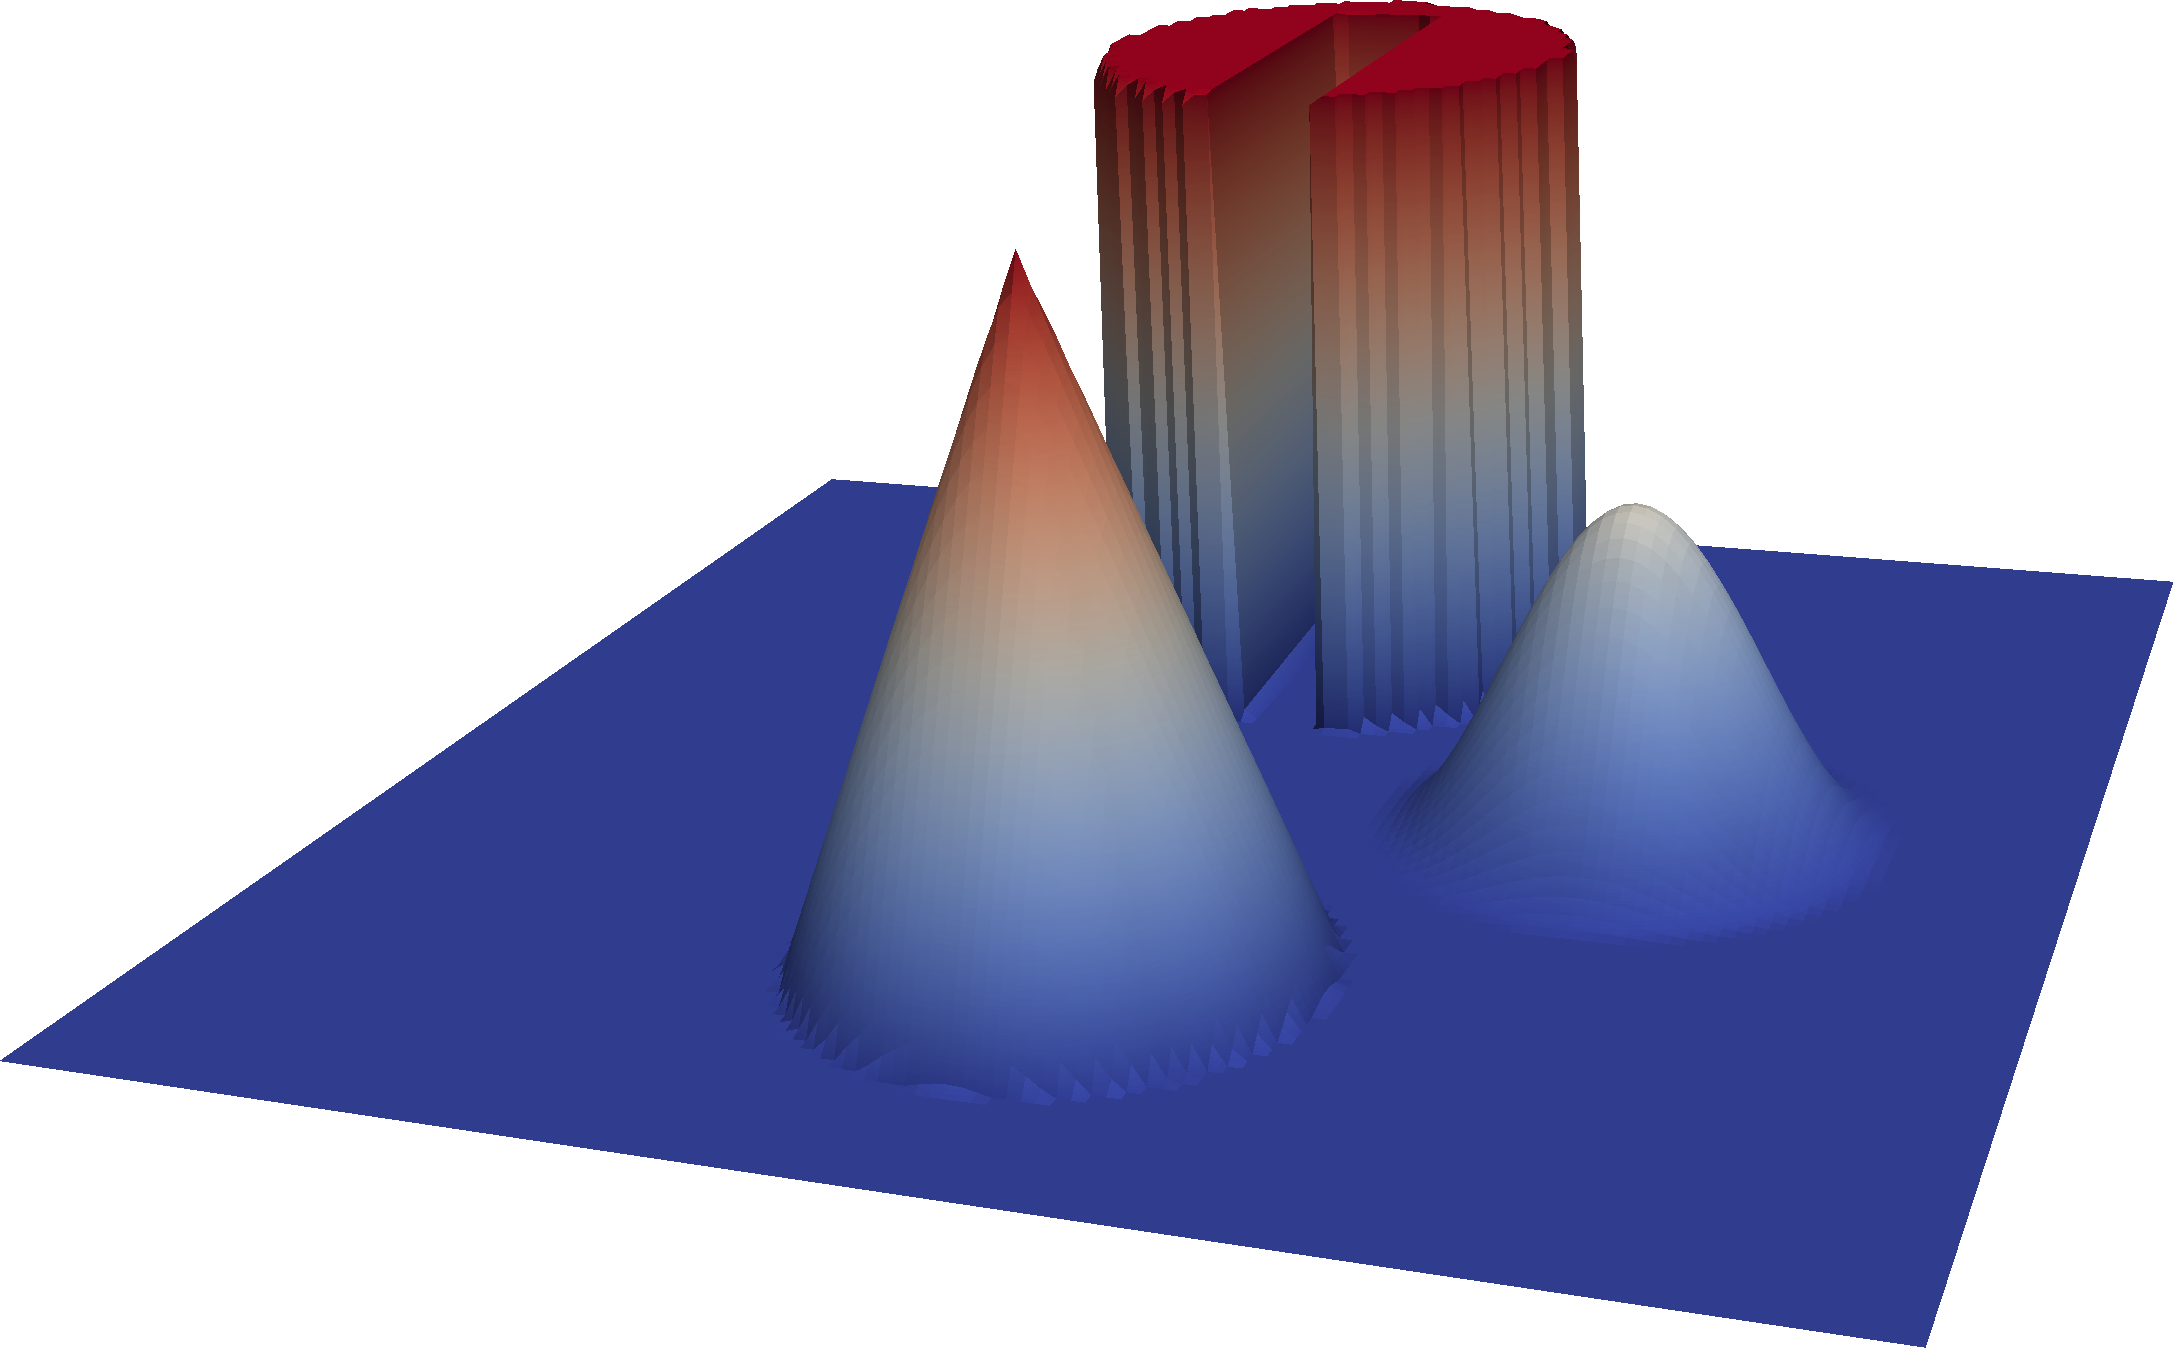
\includegraphics[width= 0.5\textwidth]{Figures/solidbodyrotinit.png}
    \caption{%
        Initial conditions for the solid body rotation test in section \ref{ss:sbrt}.
        }%
   \label{fig:sbrotinit}
\end{figure}
  
\begin{figure}
     \centering  
    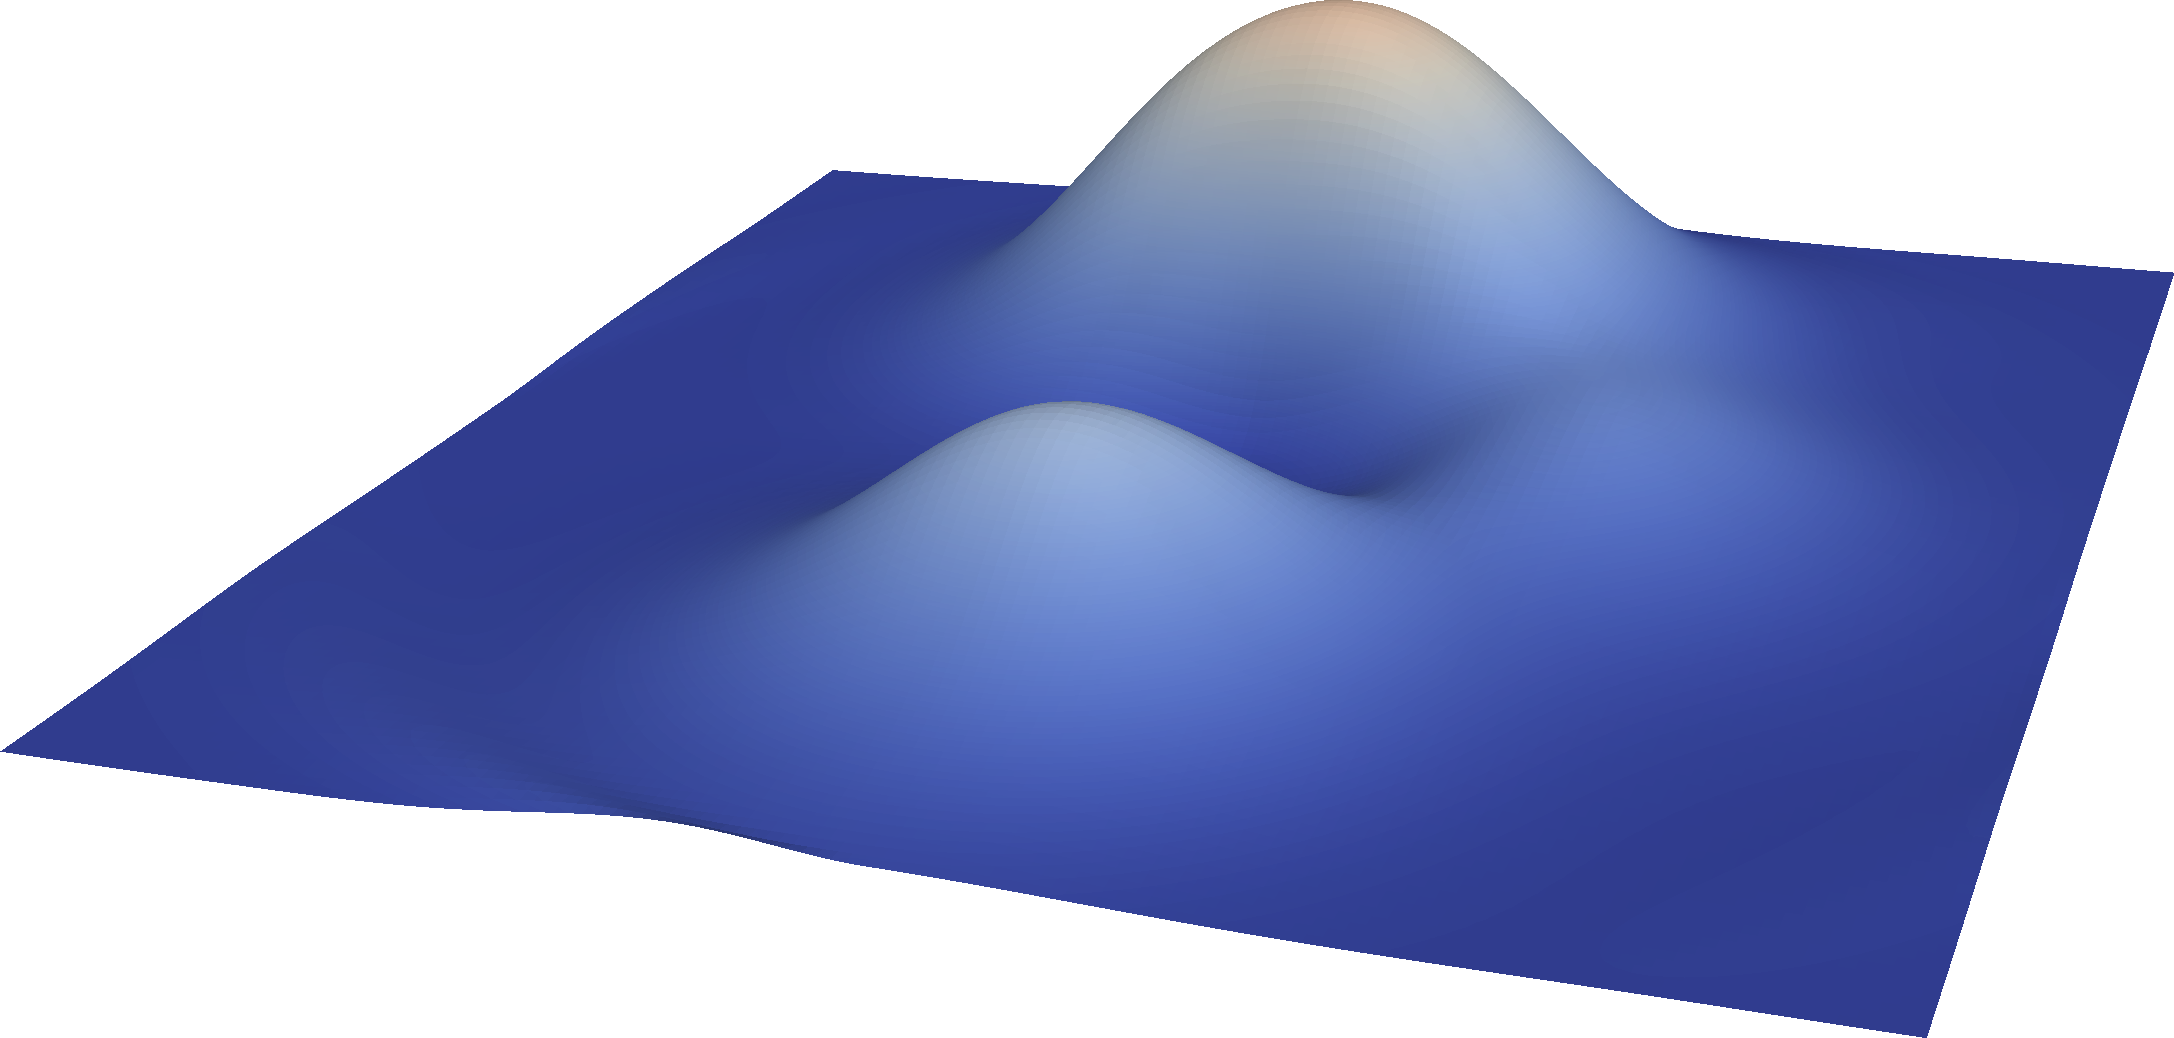
\includegraphics[width= 0.5\textwidth]{Figures/solidbodyrotup.png}
    \caption{%
        Result with the upwind method.
        }%
   \label{fig:sbrotup}
\end{figure}

\begin{figure}
     \centering  
    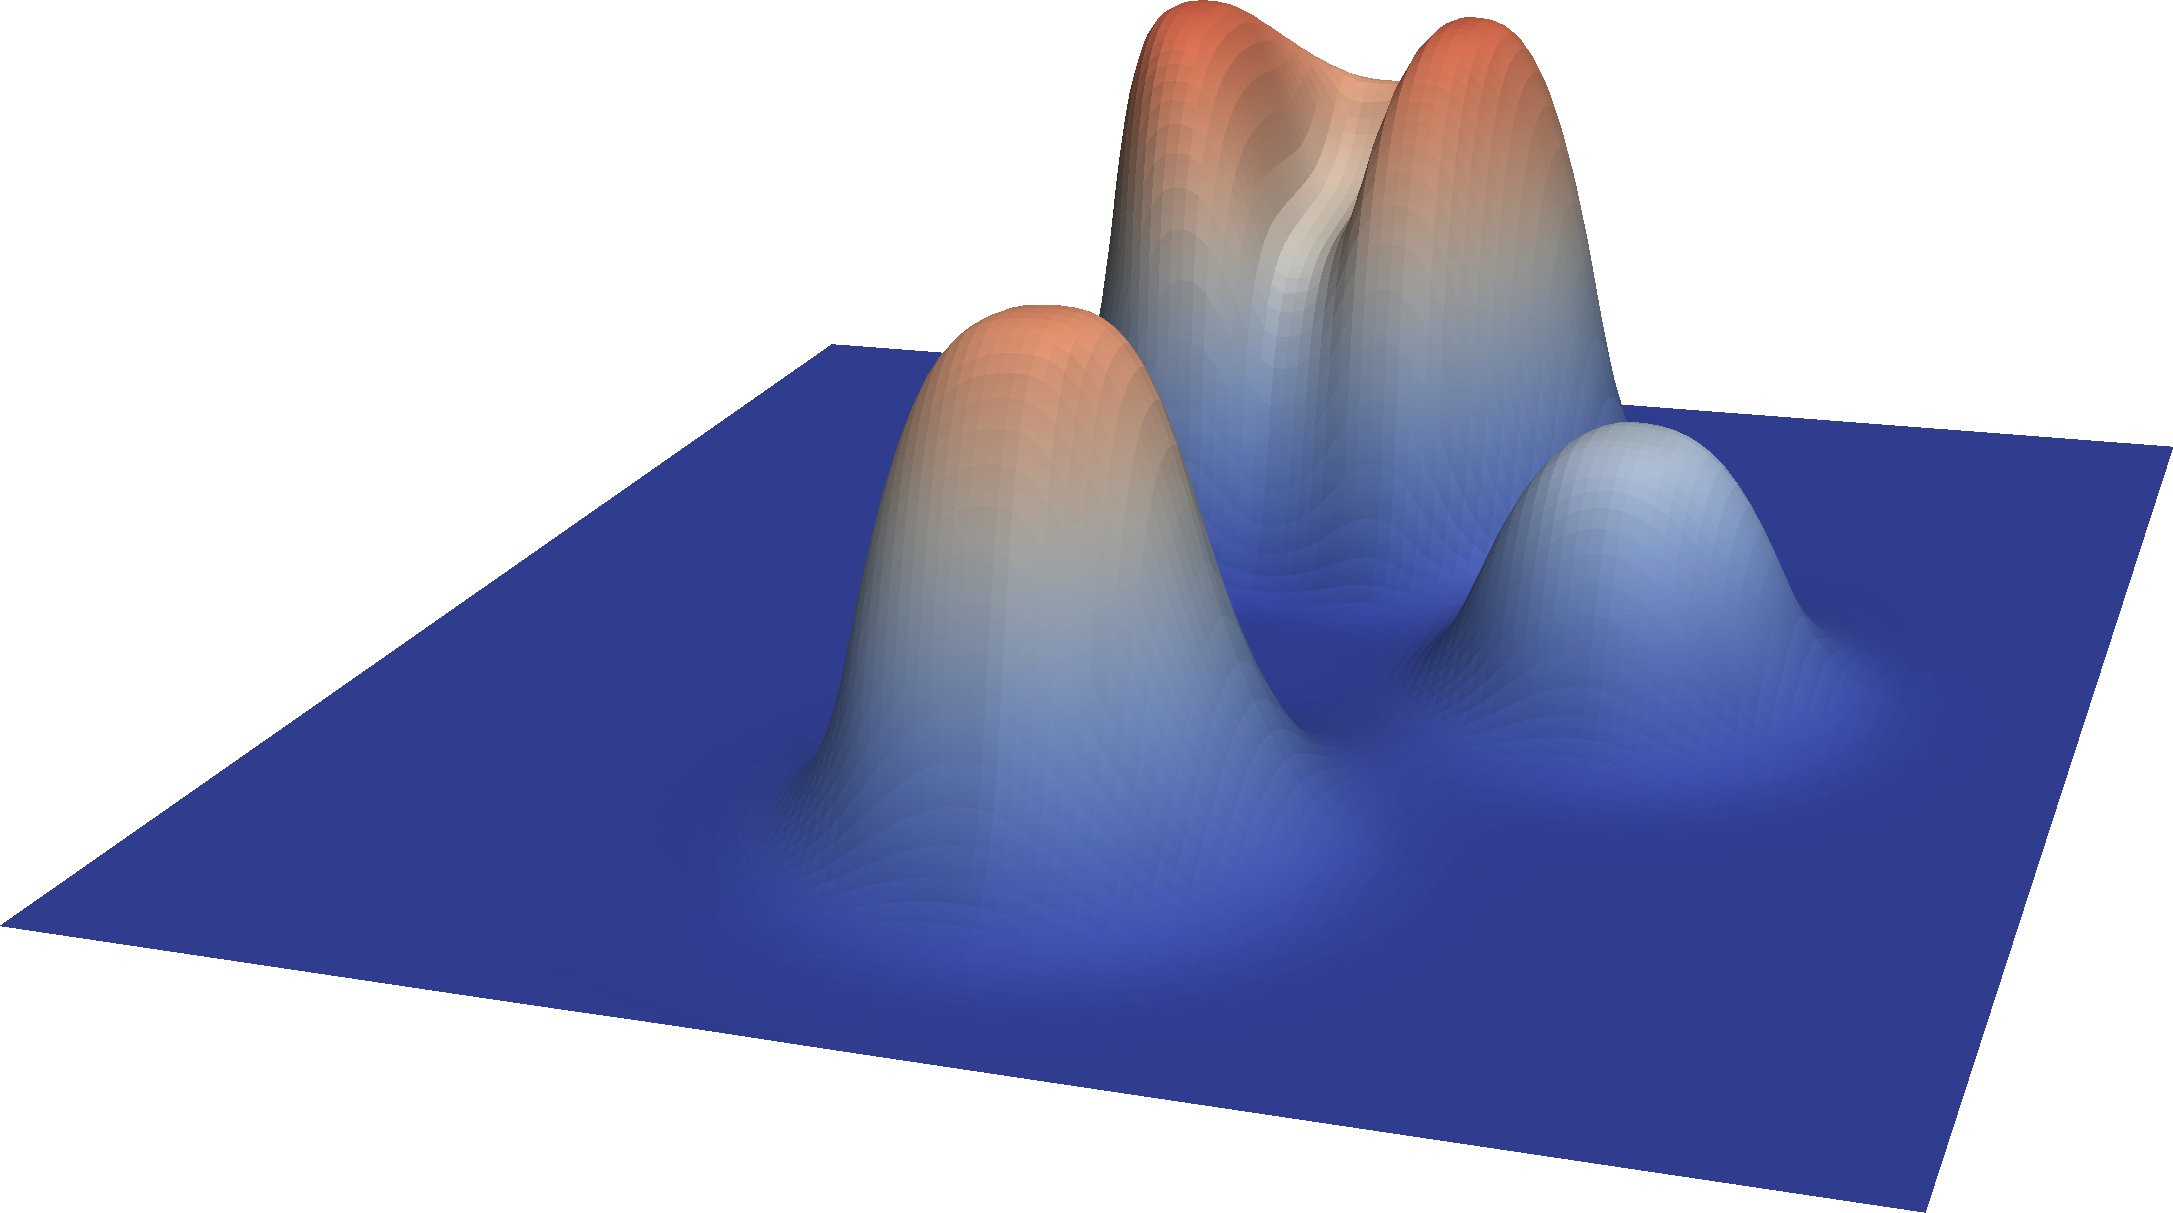
\includegraphics[width= 0.5\textwidth]{Figures/solidbodyrotminmod.png}
    \caption{%
        Result of the high resolution method with the minmod limiter.
        }%
   \label{fig:sbrotmm}
\end{figure}

\begin{figure}
     \centering  
    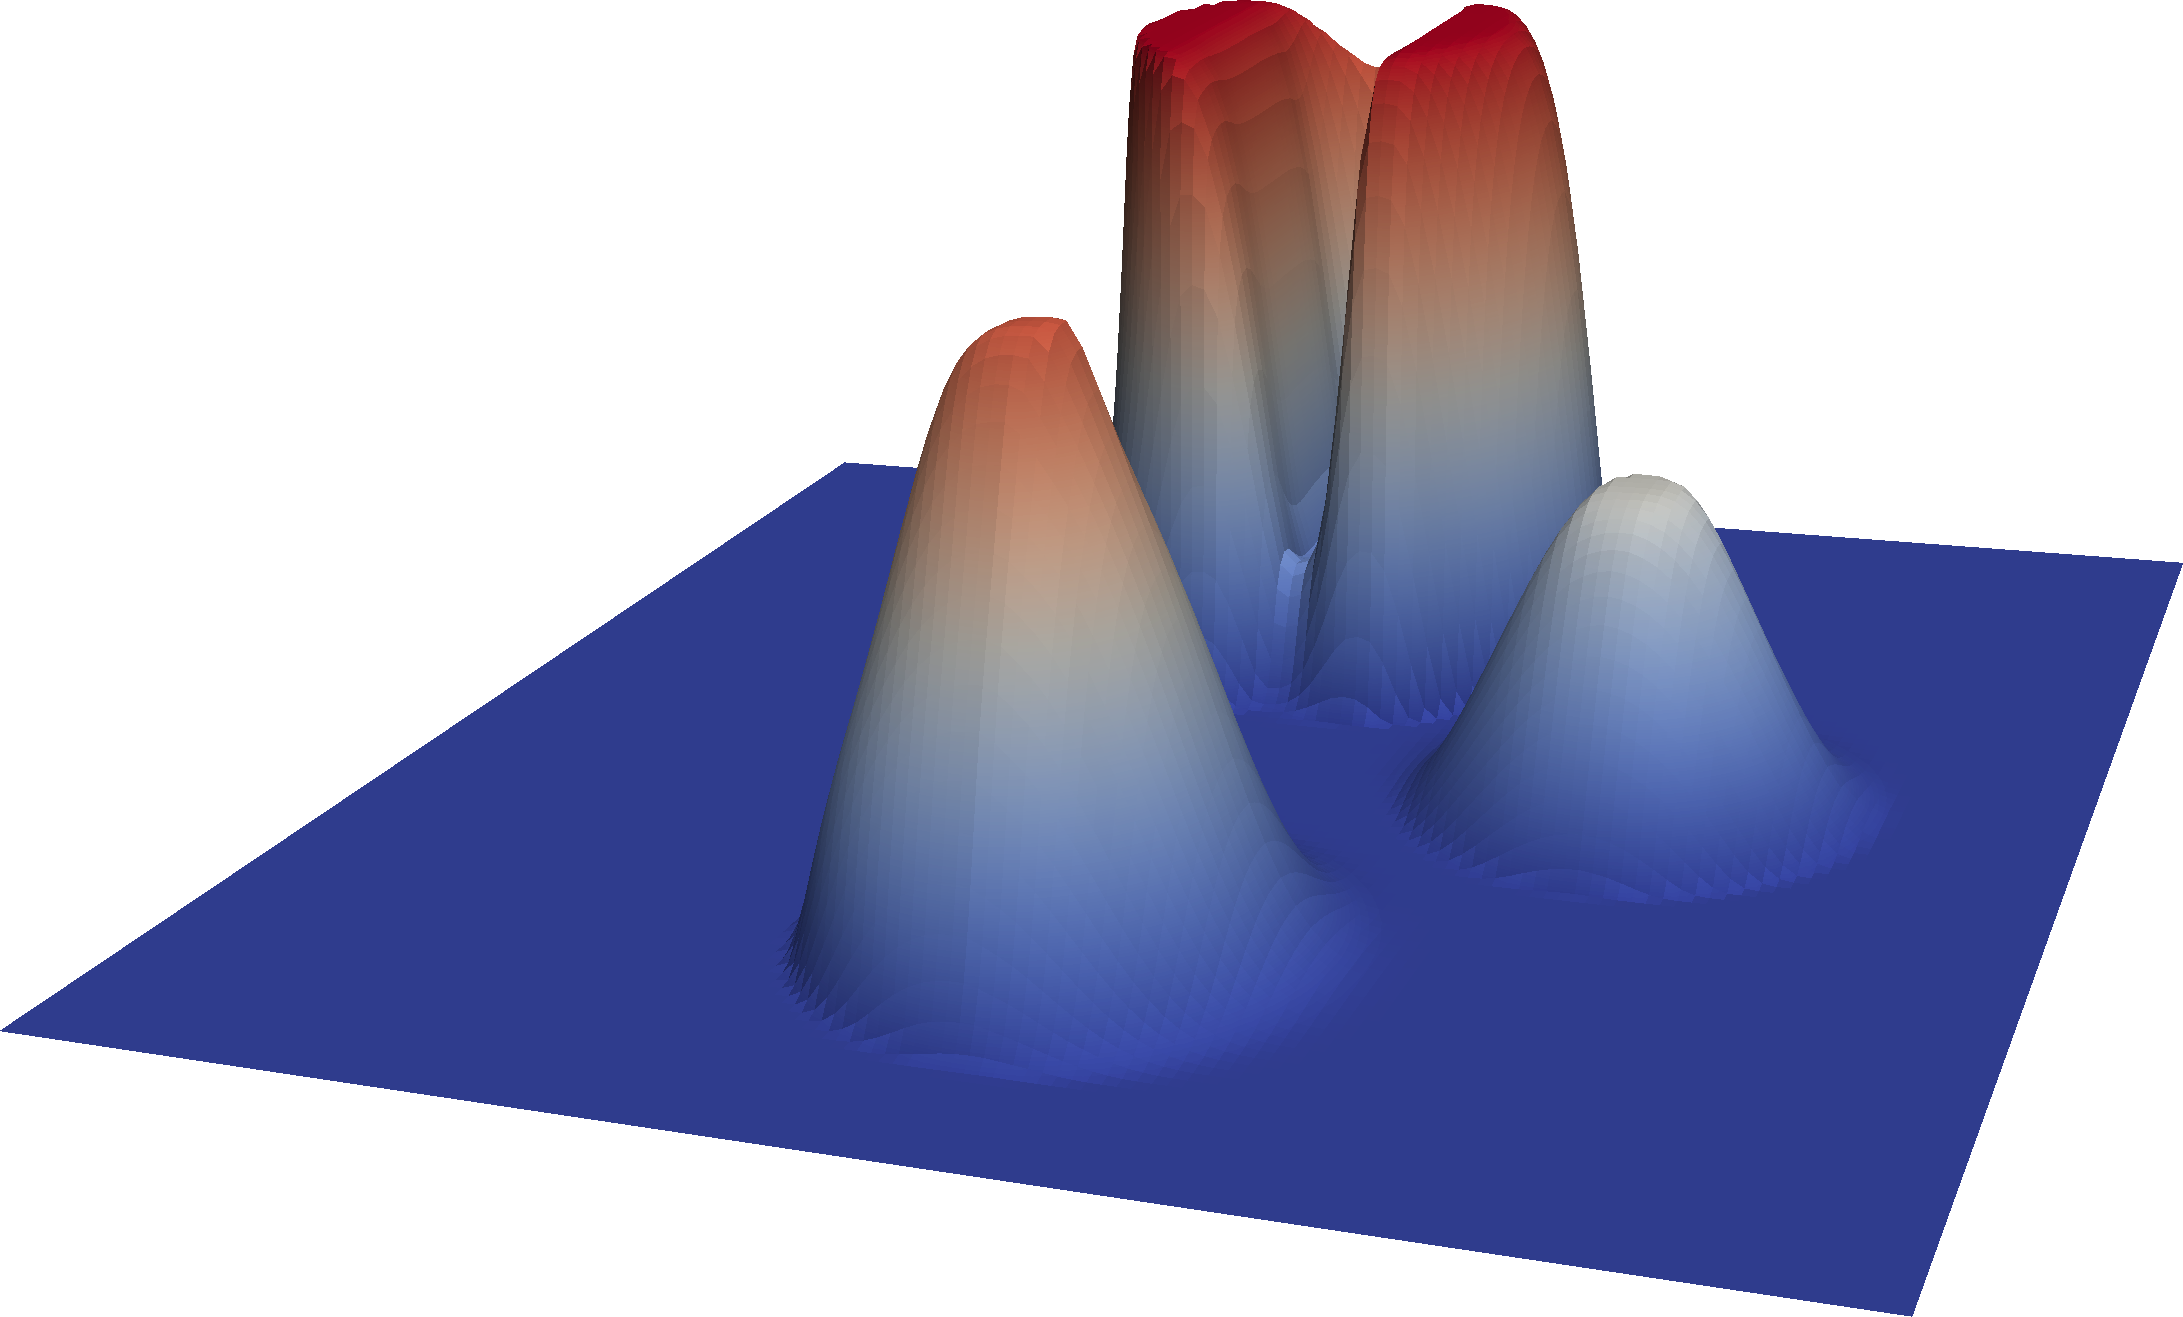
\includegraphics[width= 0.5\textwidth]{Figures/solidbodyrotmc.png}
    \caption{%
        Result of the high resolution method with the MC-limiter.
        }%
   \label{fig:sbrotmc}
\end{figure}


\begin{figure}
     \centering  
    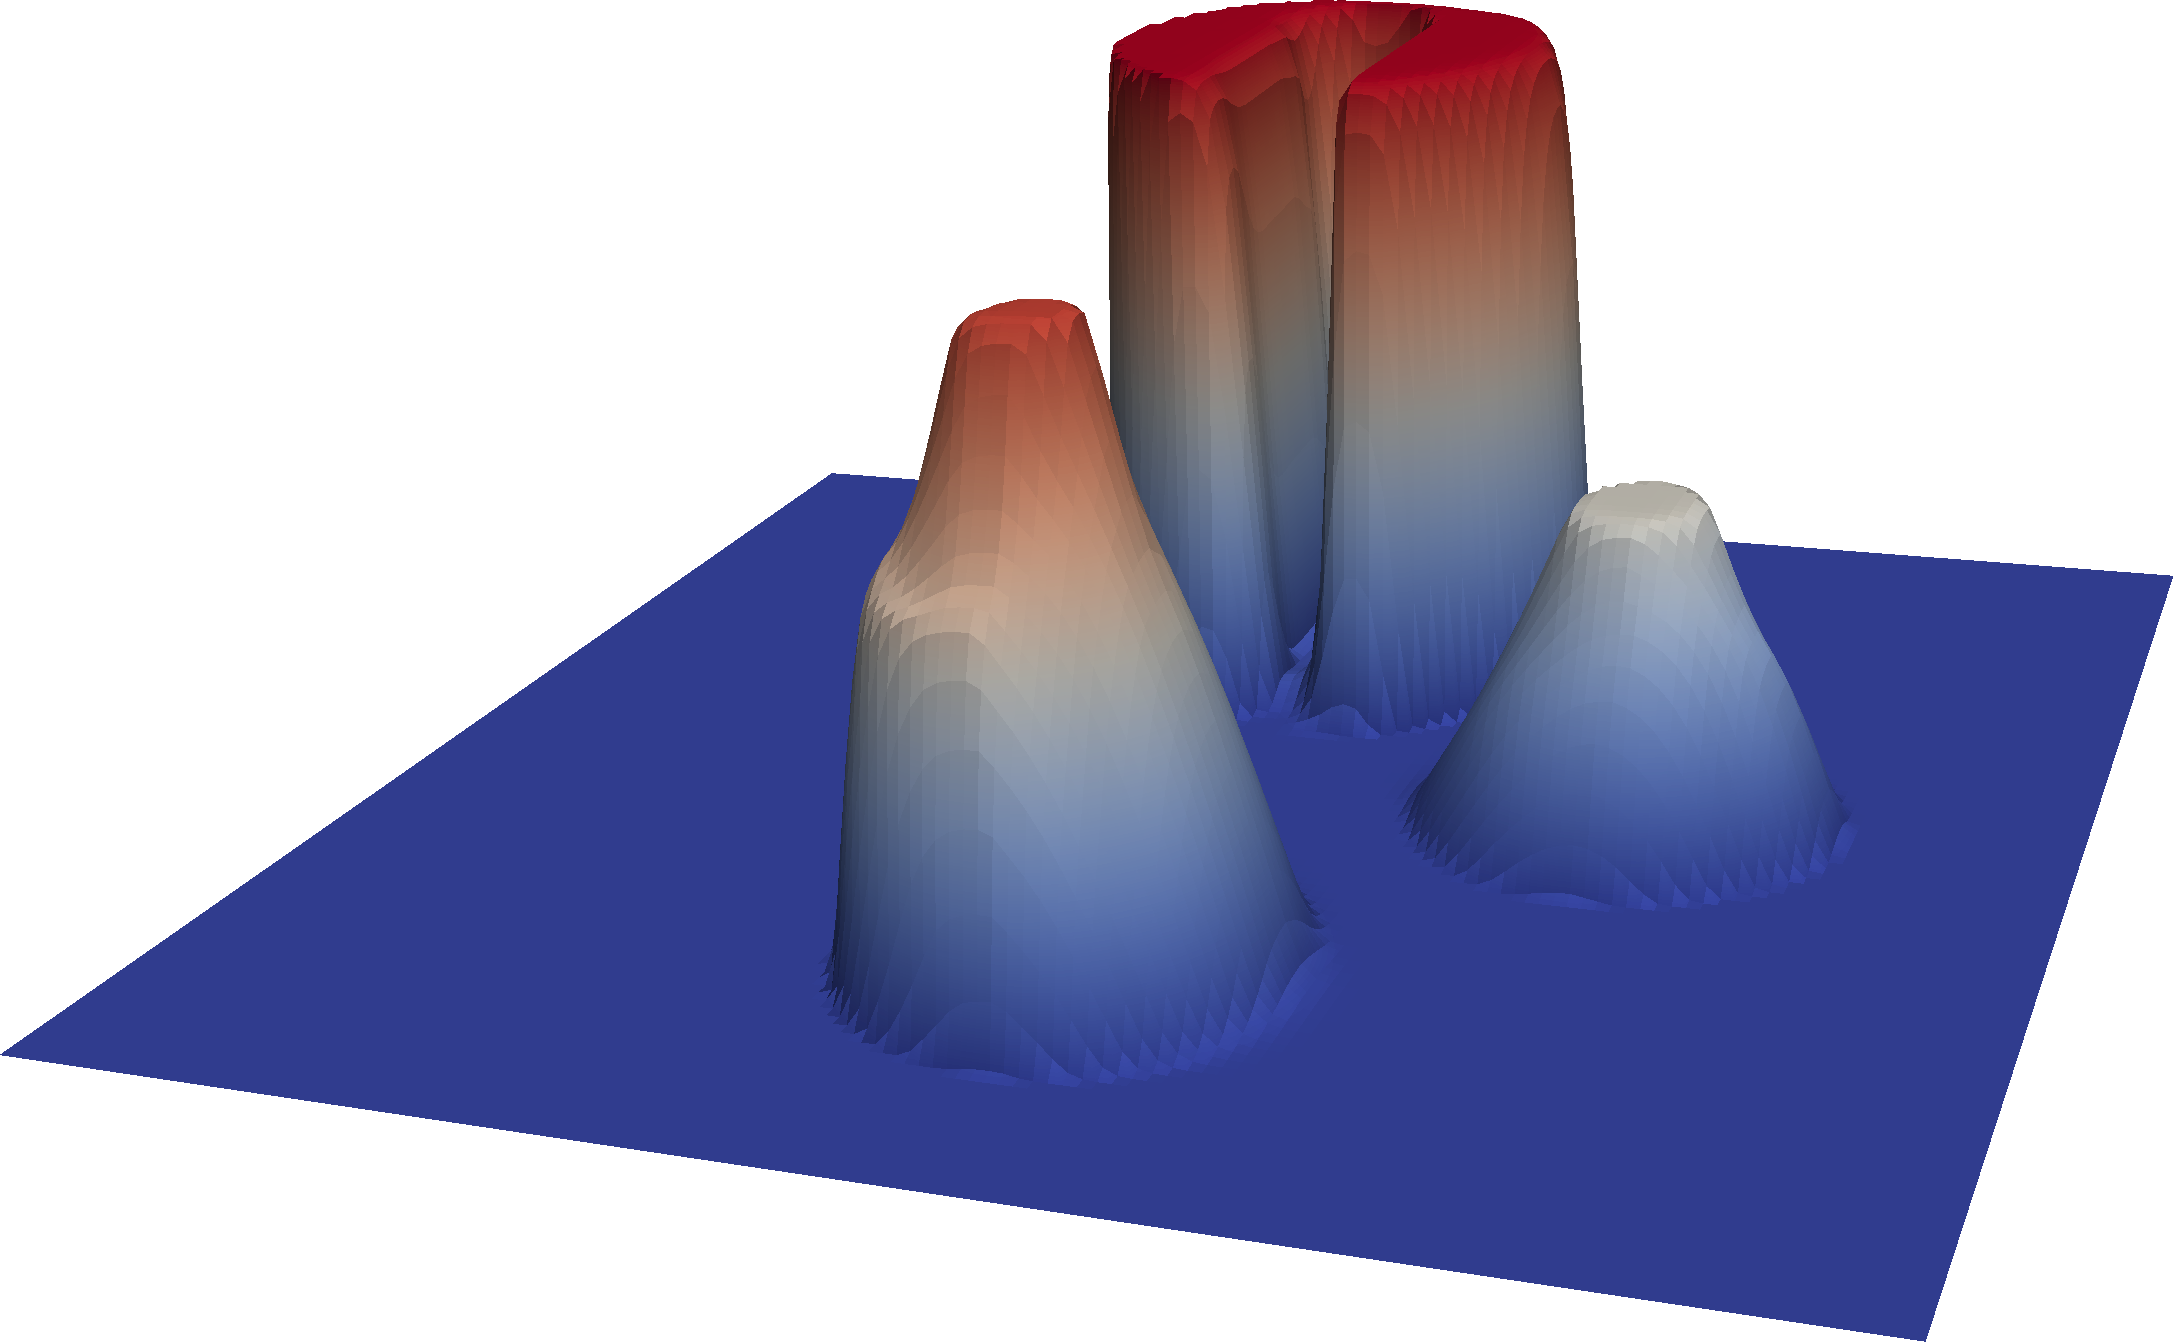
\includegraphics[width= 0.5\textwidth]{Figures/solidbodyrotsb.png}
    \caption{%
        Result of the high resolution method with the superbee limiter.
        }%
   \label{fig:sbrotsb}
\end{figure}


\begin{table}
\centering
\begin{tabular}{l|r|r}
Method & $L_1$ error & $L_2$ error \\
\hline
Upwind & 0.0948 & 0.1798 \\
Minmod & 0.0405 & 0.1142 \\
MC & 0.0202 &  0.0768 \\
Superbee & 0.0134 &  0.0540
\end{tabular}
\caption{Results of the solid body rotation test in section \ref{ss:sbrt} with various limiters.}
\label{tab:sbrt}
\end{table}
In table \ref{tab:sbrt} we see that the superbee limiter generates the smallest error, while the first-order upwind method creates the largest error. However in figure~\ref{fig:sbrotsb} we see that the cone gets a bit distorted with the superbee limiter, whereas the MC-Limiter produces a much better result as seen in figure~\ref{fig:sbrotmc}, also the top of the hump remains smooth. With the first-order Upwind method as well as the Minmod-Limiter we see significant numerical diffusion in figures~\ref{fig:sbrotup} and ~\ref{fig:sbrotmm}.

\begin{description}[font=\sffamily, font=\normalsize]
  \lstitem{void Initialize (const Settings &Settings)} Standard initialize function.
  \lstitem{void ReadInput (const std::string InputFileName)} Standard read input functions, selects the scheme via \$scheme from Advection.opi. Options are Upwind, Minmod, MC and Superbee.
  \lstitem{void Advect (Storage3D< T, rank > &Field, const Velocities &Vel, const BoundaryConditions &BC, const double dx, const double dt, const int tStep)} Advects data stored in \cmethod{Storage3D} if the type \cmethod{T} is \cmethod{double}, \cmethod{dVector3}, \cmethod{Quaternion} or \cmethod{vStress} according to the velocity field in \cmethod{Vel} with the time step \cmethod{dt} and the grid width \cmethod{dx}. In order to use the Strang splitting the number of the timestep  \cmethod{tStep} has to be provided.
  \lstitem{void Advect (PhaseField &Phase, const Velocities &Vel, const BoundaryConditions &BC, const double dx, const double dt, const int tStep)} Specialization for the Phasefield class.
  \lstitem{void Advect (Composition &Cx, const Velocities &Vel, const BoundaryConditions &BC, const double dx, const double dt, const int tStep)} Specialization for the Composition class.
  \lstitem{void Advect (Temperature &Tx, const Velocities &Vel, const BoundaryConditions &BC, const double dx, const double dt, const int tStep)} Specialization for the Temperature class.
  \lstitem{void Advect (ElasticProperties &EP, const Velocities &Vel, const BoundaryConditions &BC, const double dx, const double dt, const int tStep)} Specialization for the ElasticProperties class.
  \lstitem{void Advect (Orientations &OR, const Velocities &Vel, const BoundaryConditions &BC, const double dx, const double dt, const int tStep)} Specialization for the Orientations class.
  \lstitem{void Advect (Plasticity &PL, PhaseField &Phase, const Velocities &Vel, const BoundaryConditions &BC, const double dx, const double dt, const int tStep)} Specialization for the Plasticity class.
\end{description}

% ----------------------------------------------------------------
\CallGraphSettings

\begin{figure}
\centering
\begin{tikzpicture}[framed, node distance = 2cm, auto]
    \node [block] (constructor) {constructor};
    \node [block, below of=constructor] (init) {Initialize()};
    \node [block, below of=init] (input) {ReadInput(Filename)};
 
    % Draw edges
    \path [line] (constructor) -- (init);
    \path [line] (init) -- (input);
\end{tikzpicture}
\caption{In and output for module \nameref{sec:module_advection}}
\end{figure}
